\chapter{Data samples and simulation}
\begin{section}{Data}

The dataset used in this search corresponds to 35.9~\ifb of proton-proton collisions at $\sqrt{s} = 13~\TeV$ collected by the CMS detector over the year 2016.
This is a subset of the 40.8~\ifb delivered by the LHC and selected to correspond to when all sub-detectors were fully-operational.
A plot of the cumulative delivered and recorded integrated luminosity by the LHC and CMS, respectively, is shown in~\ref{fig:lumi_2016}. 

The data samples used in this analysis are shown in Table~\ref{tab:data_samples}.
The \texttt{JetHT} datasets are primarily used to populate the analysis search region with events, while the \texttt{Single Electron} and \texttt{Single Muon} datasets are primarily used for trigger efficiency studies.

\begin{figure}[tbp!]
\begin{center}
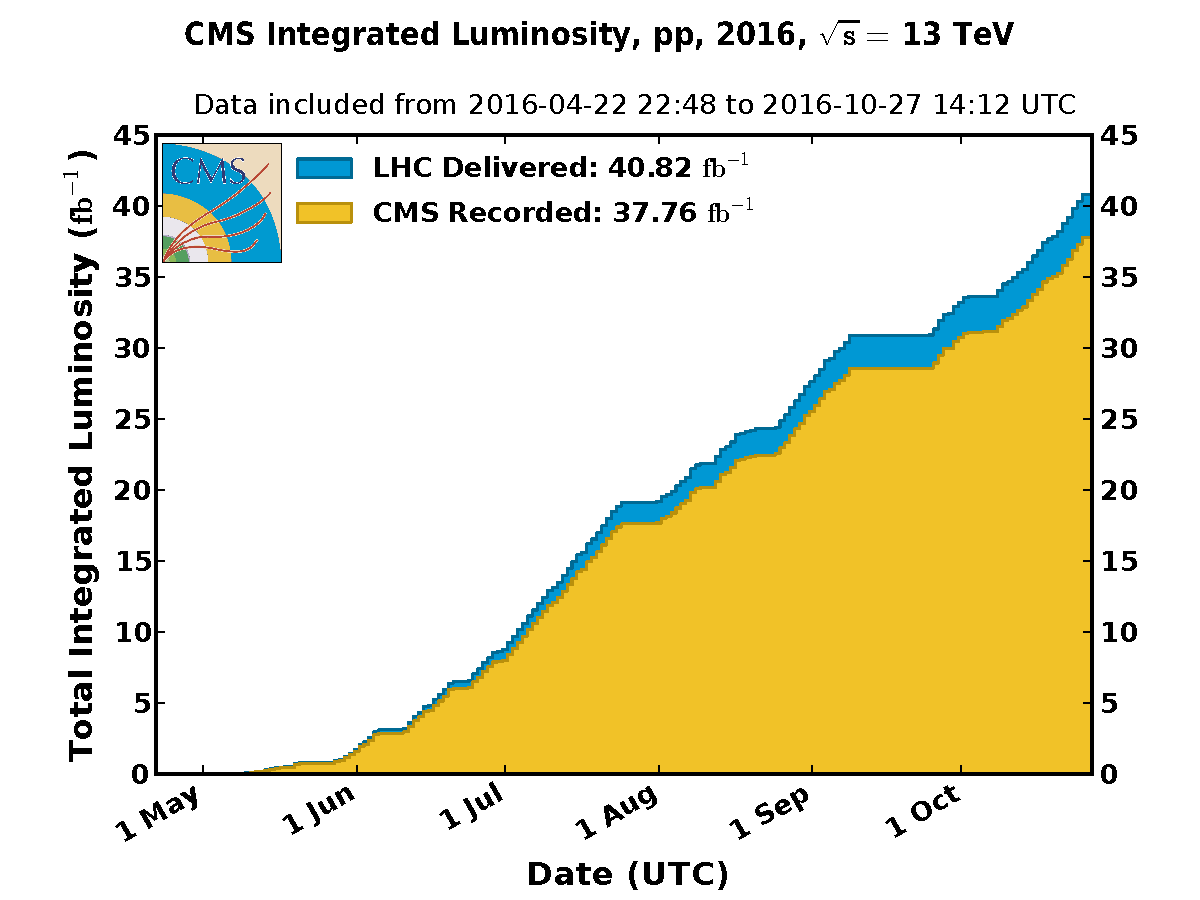
\includegraphics[angle=0,width=0.80\columnwidth]{fig/lumi_2016.pdf}
\end{center}
\caption{Delivered and recorded integrated luminosity by the LHC and CMS, respectively, over 2016.~\cite{lumi_2016}}
\label{fig:lumi_2016}
\end{figure}

\begin{table}[bt!]
\begin{center}
\begin{tabular}{l}
\hline \hline
Dataset name                                        \\ 
\hline
/JetHT/Run2016B-03Feb2017\_ver2-v2/MINIAOD          \\
/JetHT/Run2016C-03Feb2017-v1/MINIAOD                \\
/JetHT/Run2016D-03Feb2017-v1/MINIAOD                \\
/JetHT/Run2016E-03Feb2017-v1/MINIAOD                \\
/JetHT/Run2016F-03Feb2017-v1/MINIAOD                \\
/JetHT/Run2016G-03Feb2017-v1/MINIAOD                \\
/JetHT/Run2016H-03Feb2017\_ver2-v1/MINIAOD          \\
/JetHT/Run2016H-03Feb2017\_ver3-v1/MINIAOD          \\

/SingleElectron/Run2016B-03Feb2017\_ver2-v2/MINIAOD \\
/SingleElectron/Run2016C-03Feb2017-v1/MINIAOD       \\
/SingleElectron/Run2016D-03Feb2017-v1/MINIAOD       \\
/SingleElectron/Run2016E-03Feb2017-v1/MINIAOD       \\
/SingleElectron/Run2016F-03Feb2017-v1/MINIAOD       \\
/SingleElectron/Run2016G-03Feb2017-v1/MINIAOD       \\
/SingleElectron/Run2016H-03Feb2017\_ver2-v1/MINIAOD \\
/SingleElectron/Run2016H-03Feb2017\_ver3-v1/MINIAOD \\

/SingleMuon/Run2016B-03Feb2017\_ver2-v2/MINIAOD     \\
/SingleMuon/Run2016C-03Feb2017-v1/MINIAOD           \\
/SingleMuon/Run2016D-03Feb2017-v1/MINIAOD           \\
/SingleMuon/Run2016E-03Feb2017-v1/MINIAOD           \\
/SingleMuon/Run2016F-03Feb2017-v1/MINIAOD           \\
/SingleMuon/Run2016G-03Feb2017-v1/MINIAOD           \\
/SingleMuon/Run2016H-03Feb2017\_ver2-v1/MINIAOD     \\
/SingleMuon/Run2016H-03Feb2017\_ver3-v1/MINIAOD     \\
\hline \hline
\end{tabular}
\caption{Data samples analyzed for this analysis.
The corresponding integrated luminosity is 35.9~\ifb.}
\label{tab:data_samples}
\end{center}
\end{table}

\end{section}

\begin{section}{Monte Carlo Simulation}

Monte Carlo simulations (MC) are used to model both SM and BSM physics processes and are extremely useful in the design and optimization of the analysis stategy of new-physics searches.
These simulated samples allow for studying processes that in data would have control regions with impure and/or small sample sizes or, in the case of signal processes, may not even exist.
This allows for both the optimization and validation of the (signal-plus-)background prediction methods, as the sensitivity of the analysis to particular signal models can be estimated and pathologies in the prediction methodology can be unearthed and investigated.
Additionally, the simulated samples can be used to help commision and understand the collected data by comparing expectations from simulation to what is actually observed, particularly in the initial data taking periods.

\begin{subsection}{Background Samples}

The \MGatNLO~2.2.2 event generator is used in leading-order (LO) mode~\cite{Alwall:2014hca,Alwall:2007fs} to generate the
\ttbar, quantum chromodynamics multijet (QCD), \Wjets and Drell--Yan background processes with extra partons, while the \ttW, \ttZ, \tttt, and $t$-channel single top quark production backgrounds are generated with \MGatNLO~2.2.2 in next-to-leading order (NLO) mode~\cite{Frederix:2012ps}.
The \POWHEG~2.0 event generator~\cite{Nason:2004rx,Frixione:2007vw,Alioli:2010xd} is used to generate the $\mathrm{tW}$, $\mathrm{\bar{t}W}$, and $s$-channel single top quark processes at NLO precision.

The \ttbar, \Wjets, and QCD samples are generated with up to 2, 4, and 2 extra partons, respectively, and all samples are generated using a top quark mass of $172.5~\GeV$ and with the NNPDF3.0 set of parton distribution functions (PDF)~\cite{Ball:2014uwa}.
For the fragmentation and showering of partons, the generated samples are interfaced with \PYTHIA~8.205~\cite{pythia8.2} and use the CUETP8M1 tune to describe the underlying event~\cite{Skands2014}.
The detector response is simulated with \GEANTfour~\cite{Agostinelli:2002hh}, and the simulated samples are processed through the same reconstruction algorithms as the data, as discussed in Chapter~\ref{chap:reco_id}.
The background samples are normalized to the highest precision cross sections available~\cite{PhysRevLett.110.252004,Gavin:2012sy,Alioli:2009je,Re:2010bp,Frixione:2015zaa,Bevilacqua:2012em,Nagy:2001fj}.

The background samples used, along with their sample size and equivalent luminosity, are shown in Table~\ref{tab:bkg_samples}.

\begin{table}
\centering
\resizebox{\textwidth}{!}{
\begin{tabular}[tbp!]{ l rr}
\hline\hline
Simulated sample name                                                         &  Events      &  L [\ifb]   \\
\hline
TTJets\_TuneCUETP8M1\_13TeV-madgraphMLM-pythia8                               &  10,259,790  &  12.57      \\
TTJets\_SingleLeptFromT\_TuneCUETP8M1\_13TeV-madgraphMLM-pythia8              &  53,056,561  &  296.90     \\
TTJets\_SingleLeptFromTbar\_TuneCUETP8M1\_13TeV-madgraphMLM-pythia8           &  60,282,318  &  337.34     \\
TTJets\_DiLept\_TuneCUETP8M1\_13TeV-madgraphMLM-pythia8                       &  30,681,952  &  358.18     \\
TTJets\_HT-600to800\_TuneCUETP8M1\_13TeV-madgraphMLM-pythia8                  &  13,838,472  &  5,291.21   \\
TTJets\_HT-800to1200\_TuneCUETP8M1\_13TeV-madgraphMLM-pythia8                 &  10,506,985  &  9,753.77   \\
TTJets\_HT-1200to2500\_TuneCUETP8M1\_13TeV-madgraphMLM-pythia8                &  2,913,606   &  14,943.68  \\
TTJets\_HT-2500toInf\_TuneCUETP8M1\_13TeV-madgraphMLM-pythia8                 &  523,826     &  225,454.60 \\
\hline
QCD\_HT100to200\_TuneCUETP8M1\_13TeV-madgraphMLM-pythia8                      &  82,072,813  &  0.00       \\
QCD\_HT200to300\_TuneCUETP8M1\_13TeV-madgraphMLM-pythia8                      &  57,336,294  &  0.03       \\
QCD\_HT300to500\_TuneCUETP8M1\_13TeV-madgraphMLM-pythia8                      &  54,706,023  &  0.15       \\
QCD\_HT500to700\_TuneCUETP8M1\_13TeV-madgraphMLM-pythia8                      &  63,336,989  &  2.16       \\
QCD\_HT700to1000\_TuneCUETP8M1\_13TeV-madgraphMLM-pythia8                     &  45,232,792  &  6.93       \\
QCD\_HT1000to1500\_TuneCUETP8M1\_13TeV-madgraphMLM-pythia8                    &  15,314,987  &  14.39      \\
QCD\_HT1500to2000\_TuneCUETP8M1\_13TeV-madgraphMLM-pythia8                    &  11,647,431  &  95.86      \\
QCD\_HT2000toInf\_TuneCUETP8M1\_13TeV-madgraphMLM-pythia8                     &  6,004,039   &  236.19     \\
\hline
WJetsToLNu\_TuneCUETP8M1\_13TeV-madgraphMLM-pythia8                           &  28,210,241  &  0.46       \\
WJetsToLNu\_HT-100To200\_TuneCUETP8M1\_13TeV-madgraphMLM-pythia8              &  27,546,847  &  16.90      \\
WJetsToLNu\_HT-200To400\_TuneCUETP8M1\_13TeV-madgraphMLM-pythia8              &  19,851,490  &  45.57      \\
WJetsToLNu\_HT-400To600\_TuneCUETP8M1\_13TeV-madgraphMLM-pythia8              &  7,432,643   &  125.41     \\
WJetsToLNu\_HT-600To800\_TuneCUETP8M1\_13TeV-madgraphMLM-pythia8              &  18,132,628  &  1,243.62   \\
WJetsToLNu\_HT-800To1200\_TuneCUETP8M1\_13TeV-madgraphMLM-pythia8             &  1,540,354   &  231.42     \\
WJetsToLNu\_HT-1200To2500\_TuneCUETP8M1\_13TeV-madgraphMLM-pythia8            &  7,012,526   &  4,360.78   \\
WJetsToLNu\_HT-2500ToInf\_TuneCUETP8M1\_13TeV-madgraphMLM-pythia8             &  2,505,140   &  64,376.98  \\
\hline
DYJetsToLL\_M-50\_TuneCUETP8M1\_13TeV-madgraphMLM-pythia8                     &  49,190,673  &  8.17       \\
DYJetsToLL\_M-50\_HT-100to200\_TuneCUETP8M1\_13TeV-madgraphMLM-pythia8        &  7,558,769   &  44.08      \\
DYJetsToLL\_M-50\_HT-200to400\_TuneCUETP8M1\_13TeV-madgraphMLM-pythia8        &  8,683,638   &  165.14     \\
DYJetsToLL\_M-50\_HT-400to600\_TuneCUETP8M1\_13TeV-madgraphMLM-pythia8        &  396,532     &  58.65      \\
DYJetsToLL\_M-50\_HT-600to800\_TuneCUETP8M1\_13TeV-madgraphMLM-pythia8        &  8,231,815   &  4,910.15   \\
DYJetsToLL\_M-50\_HT-800to1200\_TuneCUETP8M1\_13TeV-madgraphMLM-pythia8       &  2,650,562   &  3,188.24   \\
DYJetsToLL\_M-50\_HT-1200to2500\_TuneCUETP8M1\_13TeV-madgraphMLM-pythia8      &  616,458     &  4,320.56   \\
DYJetsToLL\_M-50\_HT-2500toInf\_TuneCUETP8M1\_13TeV-madgraphMLM-pythia8       &  375,865     &  117,894.02 \\
\hline
ST\_s-channel\_4f\_leptonDecays\_13TeV-amcatnlo-pythia8\_TuneCUETP8M1         &  999,995     &  116.20     \\
ST\_t-channel\_antitop\_4f\_leptonDecays\_13TeV-powheg-pythia8\_TuneCUETP8M1  &  1,682,394   &  64.14      \\
ST\_t-channel\_top\_4f\_leptonDecays\_13TeV-powheg-pythia8\_TuneCUETP8M1      &  3,279,179   &  74.41      \\
ST\_tW\_antitop\_5f\_NoFullyHadronicDecays\_13TeV-powheg\_TuneCUETP8M1        &  5,388,666   &  343.66     \\
ST\_tW\_top\_5f\_NoFullyHadronicDecays\_13TeV-powheg\_TuneCUETP8M1            &  5,405,674   &  344.74     \\
\hline
ttHJetTobb\_M125\_13TeV\_amcatnloFXFX\_madspin\_pythia8                       &  9,823,967   &  2,957.09   \\
TTGJets\_TuneCUETP8M1\_13TeV-amcatnloFXFX-madspin-pythia8                     &  4,664,534   &  132.40     \\
TTTT\_TuneCUETP8M1\_13TeV-amcatnlo-pythia8                                    &  752,497     &  14,412.60  \\
TTWJetsToLNu\_TuneCUETP8M1\_13TeV-amcatnloFXFX-madspin-pythia8                &  252,664     &  328.75     \\
TTWJetsToQQ\_TuneCUETP8M1\_13TeV-amcatnloFXFX-madspin-pythia8                 &  833,278     &  547.03     \\
TTZToLLNuNu\_M-10\_TuneCUETP8M1\_13TeV-amcatnlo-pythia8                       &  398,596     &  340.36     \\
TTZToQQ\_TuneCUETP8M1\_13TeV-amcatnlo-pythia8                                 &  749,386     &  310.64     \\
\hline
WWTo2L2Nu\_13TeV-powheg                                                       &  1,996,585   &  163.95     \\
WZTo3LNu\_TuneCUETP8M1\_13TeV-powheg-pythia8                                  &  1,820,203   &  410.91     \\
\hline\hline
\end{tabular}
}
\caption{Simulated background samples used in this analysis with their corresponding sample size and equivalent luminosity.}
\label{tab:bkg_samples}
\end{table}

\end{subsection}

\begin{subsection}{Signal Samples}

For ease of generation and interpretation, signal samples are produced according to the Simplifed Model Spectra (SMS) paradigm~\cite{Alwall:2008ag,Alves:2011wf}, where all but one or two mass parameters in a particular decay chain are fixed.
Due to their ``simplicity'', SMS models can be interpreted generally, reducing the sensitivity of results to model specifics and allowing for results to be applicable to a wide variety of new-physics models.
Additionally, the use of SMS models results in signficantly reduced computing time for model generation, as models need to be produced by scanning across at most only two parameters.

The assumpations used in the simplified model of the \rpvDecay process, denoted as T1tbs, are given below:
\begin{itemize}
\item squarks other than the top squark are much heavier than the gluino, so they do not affect the gluino decay
\item the branching ratio of \rpvDecay is $100\%$
\item the top squark is virtual in its decay. This results in a three-body decay, so searches for dijet resonances, i.e., $\bar{\tilde{\mrm{t}}} \to \mrm{bs}$, are not applicable in this scenario.
\item the gluinos decay promptly
\end{itemize}

These assumptions correspond to a model of direct gluino pair production with each gluino decaying to a top, bottom, and strange quark. 
An example diagram of the T1tbs model is shown in Figure~\ref{fig:T1tbs_diagram}.
The only free parameter in this model is the mass of the gluino, and 11 signal models are generated between $\mglu = 1000$ and $2000~\GeV$ in steps of $100~\GeV$.

\begin{figure}[tbp!]
\begin{center}
\includegraphics[angle=0,width=0.60\columnwidth]{fig/T1tbs_diagram.png}
\end{center}
\caption{Example diagram of the T1tbs simplified model.}
\label{fig:T1tbs_diagram}
\end{figure}

These signal models are generated with up to two extra partons in leading-order mode and dynamic factorization and renormalization scales by \MGatNLO~2.2.2.
The rest of the signal sample production follows the same procedure used for the background samples, which includes the parton fragmentation and showering, simulation, and event reconstruction.
Lastly, the samples are normalized to the NLO + next-to-leading logarithmic cross sections for gluino pair production~\cite{XSecgluinogluino}.

\begin{table}
\centering
\resizebox{\textwidth}{!}{
\begin{tabular}[tbp!]{ l rrr}
\hline\hline
Dataset name                                                              &  Events  &  L [\ifb]  \\
\hline
SMS-T1tbs\_mGluino-1000\_mLSP-0\_TuneCUETP8M1\_13TeV-madgraphMLM-pythia8  &  130,281 &  400.39    \\
SMS-T1tbs\_mGluino-1100\_mLSP-0\_TuneCUETP8M1\_13TeV-madgraphMLM-pythia8  &  71,488  &  437.26    \\
SMS-T1tbs\_mGluino-1200\_mLSP-0\_TuneCUETP8M1\_13TeV-madgraphMLM-pythia8  &  50,739  &  592.46    \\
SMS-T1tbs\_mGluino-1300\_mLSP-0\_TuneCUETP8M1\_13TeV-madgraphMLM-pythia8  &  31,815  &  690.84    \\
SMS-T1tbs\_mGluino-1400\_mLSP-0\_TuneCUETP8M1\_13TeV-madgraphMLM-pythia8  &  21,392  &  845.61    \\
SMS-T1tbs\_mGluino-1500\_mLSP-0\_TuneCUETP8M1\_13TeV-madgraphMLM-pythia8  &  16,702  &  1,177.00  \\
SMS-T1tbs\_mGluino-1600\_mLSP-0\_TuneCUETP8M1\_13TeV-madgraphMLM-pythia8  &  10,101  &  1,246.92  \\
SMS-T1tbs\_mGluino-1700\_mLSP-0\_TuneCUETP8M1\_13TeV-madgraphMLM-pythia8  &  10,380  &  2,206.99  \\
SMS-T1tbs\_mGluino-1800\_mLSP-0\_TuneCUETP8M1\_13TeV-madgraphMLM-pythia8  &  9,865   &  3,572.55  \\
SMS-T1tbs\_mGluino-1900\_mLSP-0\_TuneCUETP8M1\_13TeV-madgraphMLM-pythia8  &  10,071  &  6,157.86  \\
SMS-T1tbs\_mGluino-2000\_mLSP-0\_TuneCUETP8M1\_13TeV-madgraphMLM-pythia8  &  10,556  &  10,759.60 \\
\hline\hline
\end{tabular}
}
\caption{Simulated signal samples used in this analysis with their corresponding sample size and equivalent luminosity.}
\label{tab:sig_samples}
\end{table}

\end{subsection}

\end{section}
